\section{Model Verification}
\label{section_model_varification}
In this section, START mobility model is validated on the aspects of node distribution and contact characteristics. All mobility models are implemented on Opportunistic Networking Environment (ONE)\cite{KeranenOtt-155}.

Shortest Path (SP) mobility model based on the map in Beijing is an other comparison, which is implemented by ONE.  It also moves along the map roads by Dijkstra algorithm.
The RWP model is another comparison, because it is proved to be an efficient model modeling the nodal movement in VANETs. But it takes no consideration of the node statuses and geographical distribution.

The START, SP and RWP mobility model are compared with the real trace.
In simulations, Node number is set as 4000 and scenario in area $24445\times23584 m^2$ (a sub-map of the whole area), including fourth ring roads in Beijing. The simulation time is three hours and the warm up time for reports is one hour, so that the nodal movement and position will not be affected by its initial position. The communication range is $200m$.

\subsection{Traces and distribution of nodes}

Trace samples and their snapshots are demonstrated in this section, shown as fig. \ref{figure_tracesample} and fig.\ref{figure_trace_snapshots}.




Fig.\ref{figure_tracesample} shows the trace in one day. The trace of the real data and START only cover some part of the area, while the trace of SP and RWP almost go through the whole area. Because SP and RWP will select a destination randomly, while START takes the associations between current region and destinations into consideration which satisfies the movement rules of taxis.

\begin{figure}[!h]
\centering
\hspace{0.in}
\subfigure[Real Trace]{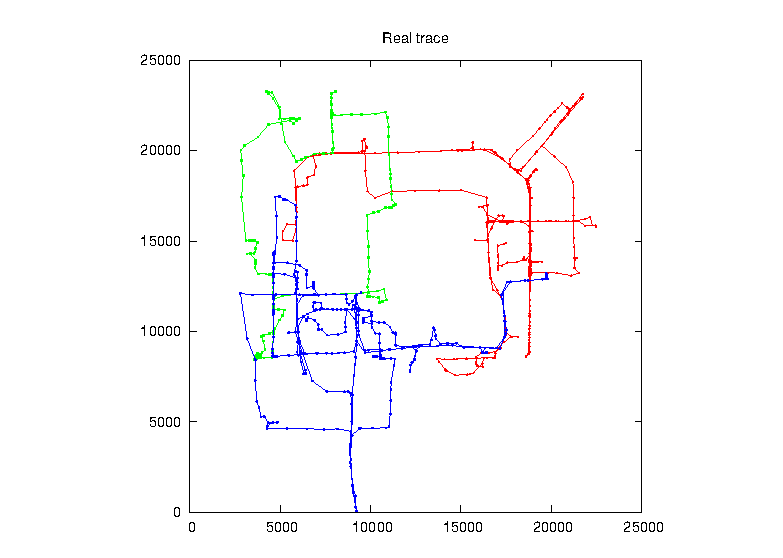
\includegraphics[width=0.23\textwidth]{figures_201103/Evaluation/trace_real.eps}}
\hspace{0.0in}
\subfigure[START]{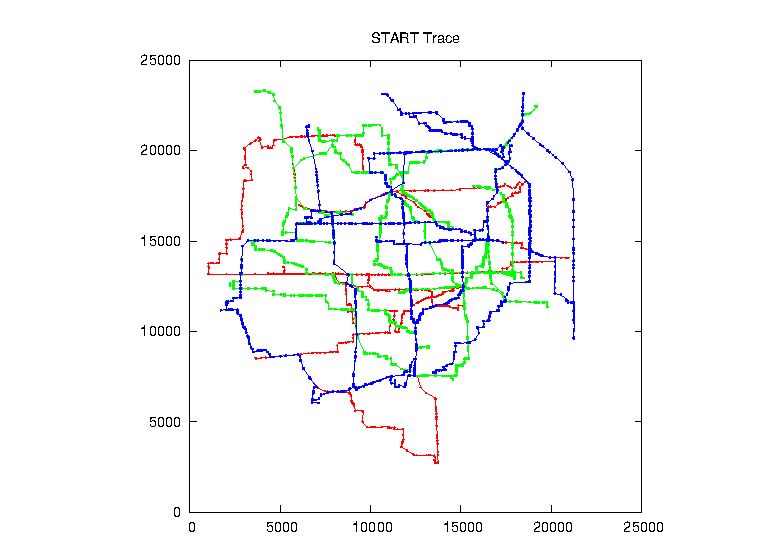
\includegraphics[width=0.23\textwidth]{figures_201103/Evaluation/trace_start.eps}}
\hspace{0.0in}
\subfigure[SP]{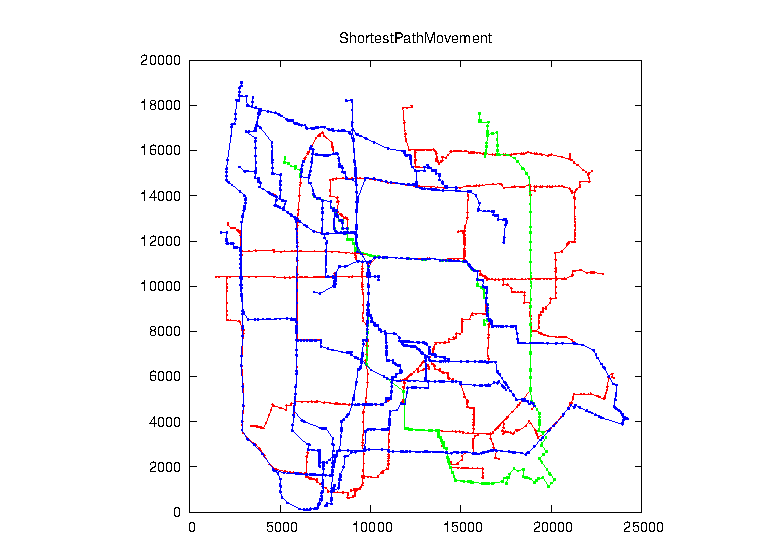
\includegraphics[width=0.23\textwidth]{figures_201103/Evaluation/trace_sp.eps}}
\hspace{0.in}
\subfigure[RWP]{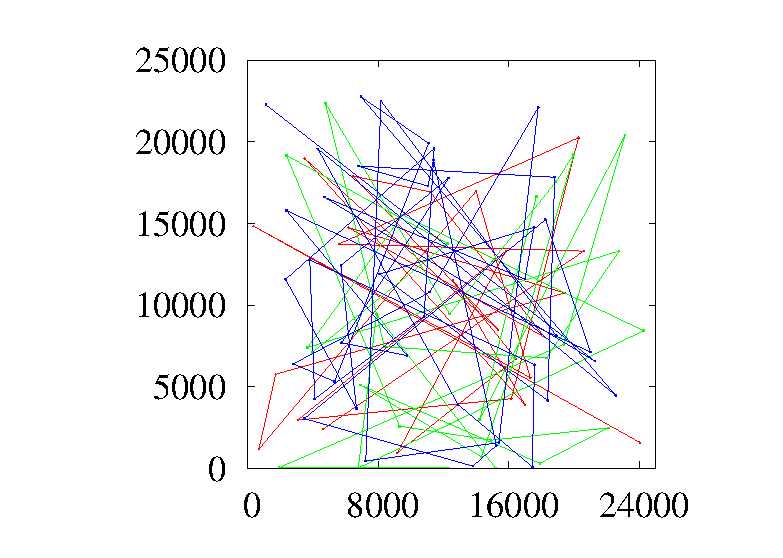
\includegraphics[width=0.23\textwidth]{figures_201103/Evaluation/trace_rwp.eps}}
\caption{Trace samples}\label{figure_tracesample}
\end{figure}

From fig.\ref{figure_trace_snapshots}, Real trace START and SP mobility model exhibit the road structure. However, the node distribution of RWP is much uniform.
As to START, the destination section process decides that it tends to select a destination in the regions with higher load/drop event probability.
Therefore, with the decline of the randomness,the snapshot of START become much clear and centralized.
\begin{figure}[!h]
\centering
\subfigure[Real Trace]{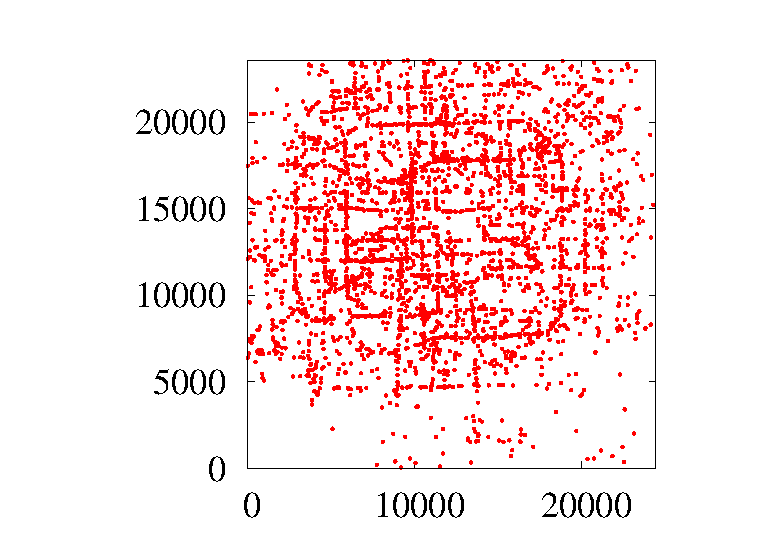
\includegraphics[width=0.23\textwidth]{figures_201103/Evaluation/sample/tracesample.eps}}
\vspace{0.in}
\hspace{0.0in}
\subfigure[START]{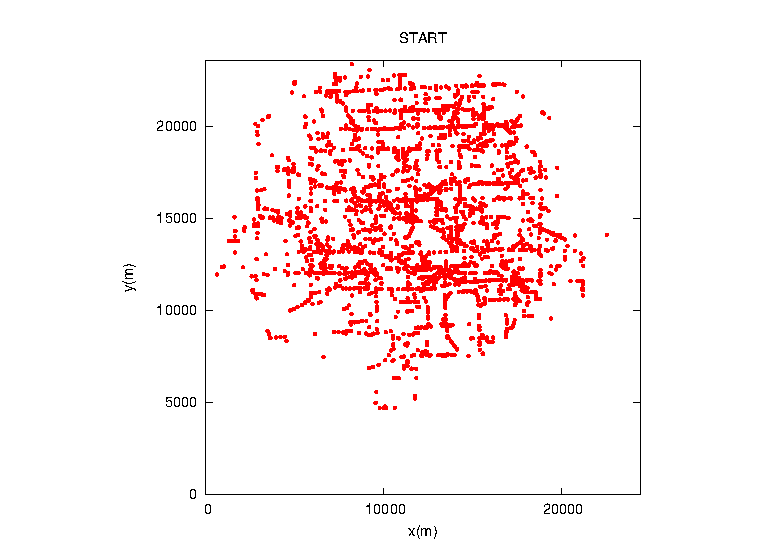
\includegraphics[width=0.23\textwidth]{figures_201103/Evaluation/sample/startsample.eps}}
\vspace{0.in}
\hspace{0.0in}
\subfigure[SP]{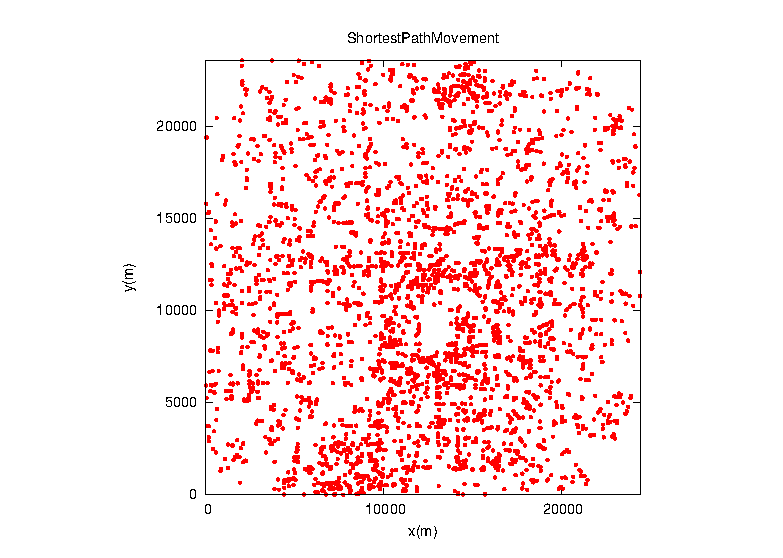
\includegraphics[width=0.23\textwidth]{figures_201103/Evaluation/sample/spsample.eps}}
\vspace{0.in}
\hspace{0.0in}
\subfigure[RWP]{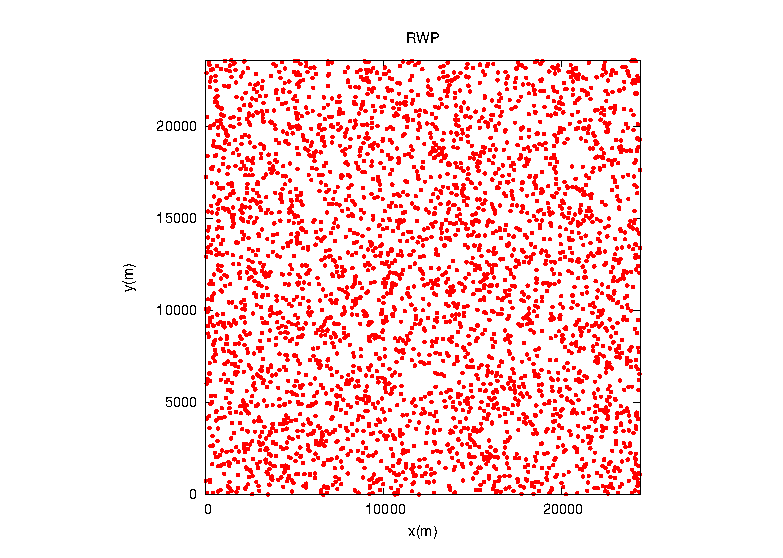
\includegraphics[width=0.23\textwidth]{figures_201103/Evaluation/sample/rwpsample.eps}}
\caption{Trace snapshots}\label{figure_trace_snapshots}
\end{figure}



\subsection{Contacts characteristics}

The contact time and inter contact time are evaluated as the indicators to validate the similarity. The speed range of RWP and SP need to be configured. To ensure the accuracy, we choose three speed range $[0,44.4]m/s$,$[0,33.3]m/s$ and $[0,22.2]m/s$, that is, the upper bounds of speed are 80,120,160 $km/h$.


\begin{figure}
\centering
\subfigure[cumulative contact time distribution]{
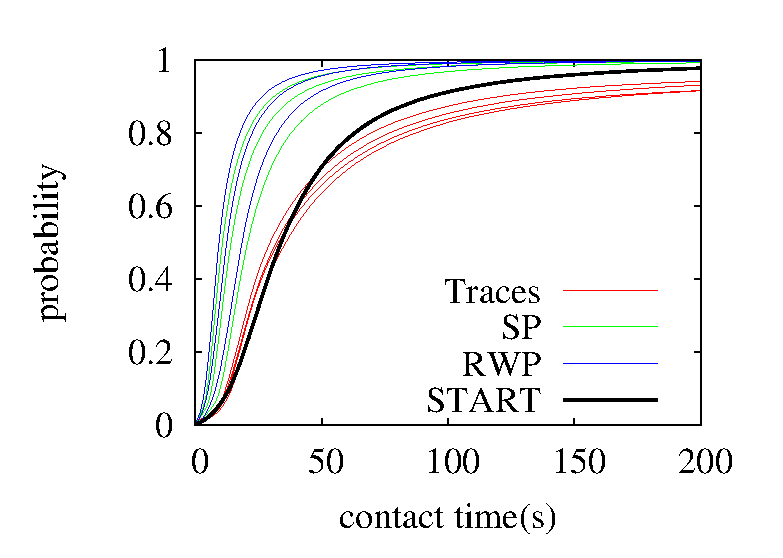
\includegraphics[width=0.3\textwidth]{figures_201103/Evaluation/contact/ct_ccdf.eps}
}
\subfigure[cumulative inter contact time distribution]{
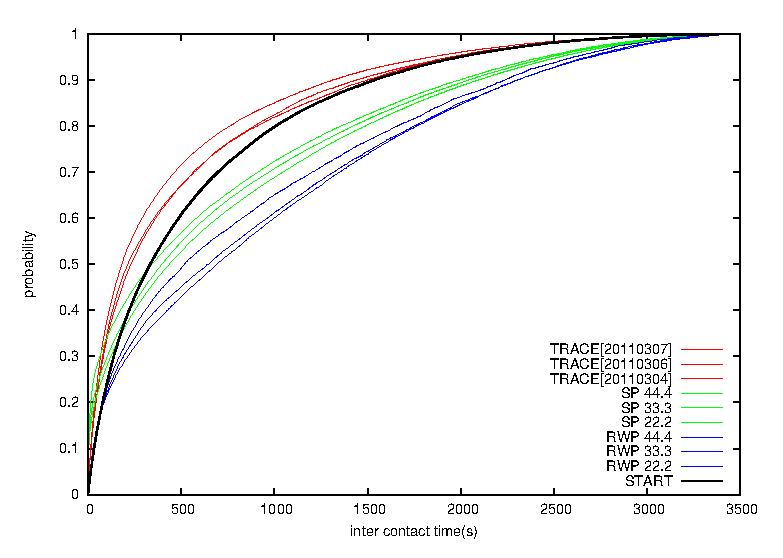
\includegraphics[width=0.3\textwidth]{figures_201103/Evaluation/contact/ict_ccdf.eps}
}
\caption{Contact time, inter contact time distribution}\label{figure_contacts}
\end{figure}


\begin{figure}
\centering
\subfigure[time vs. total contact time]{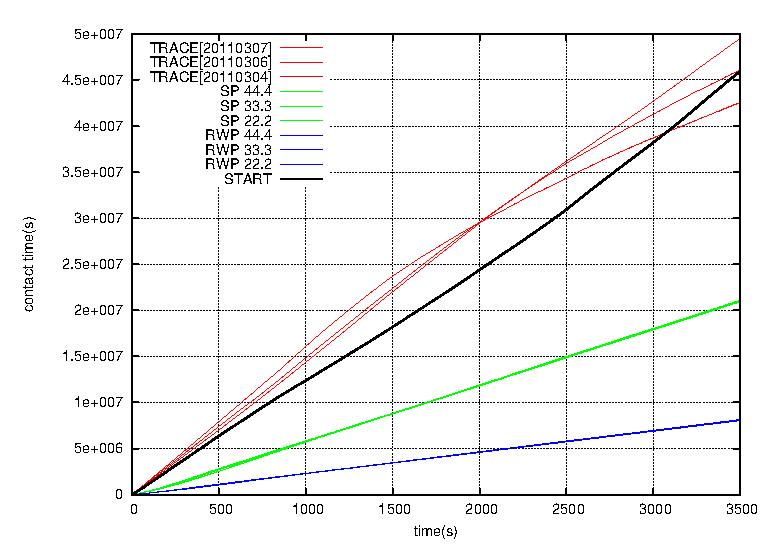
\includegraphics[width=0.23\textwidth]{figures_201103/Evaluation/contact/tc.eps}}
\subfigure[time vs. total contact time in logscale]{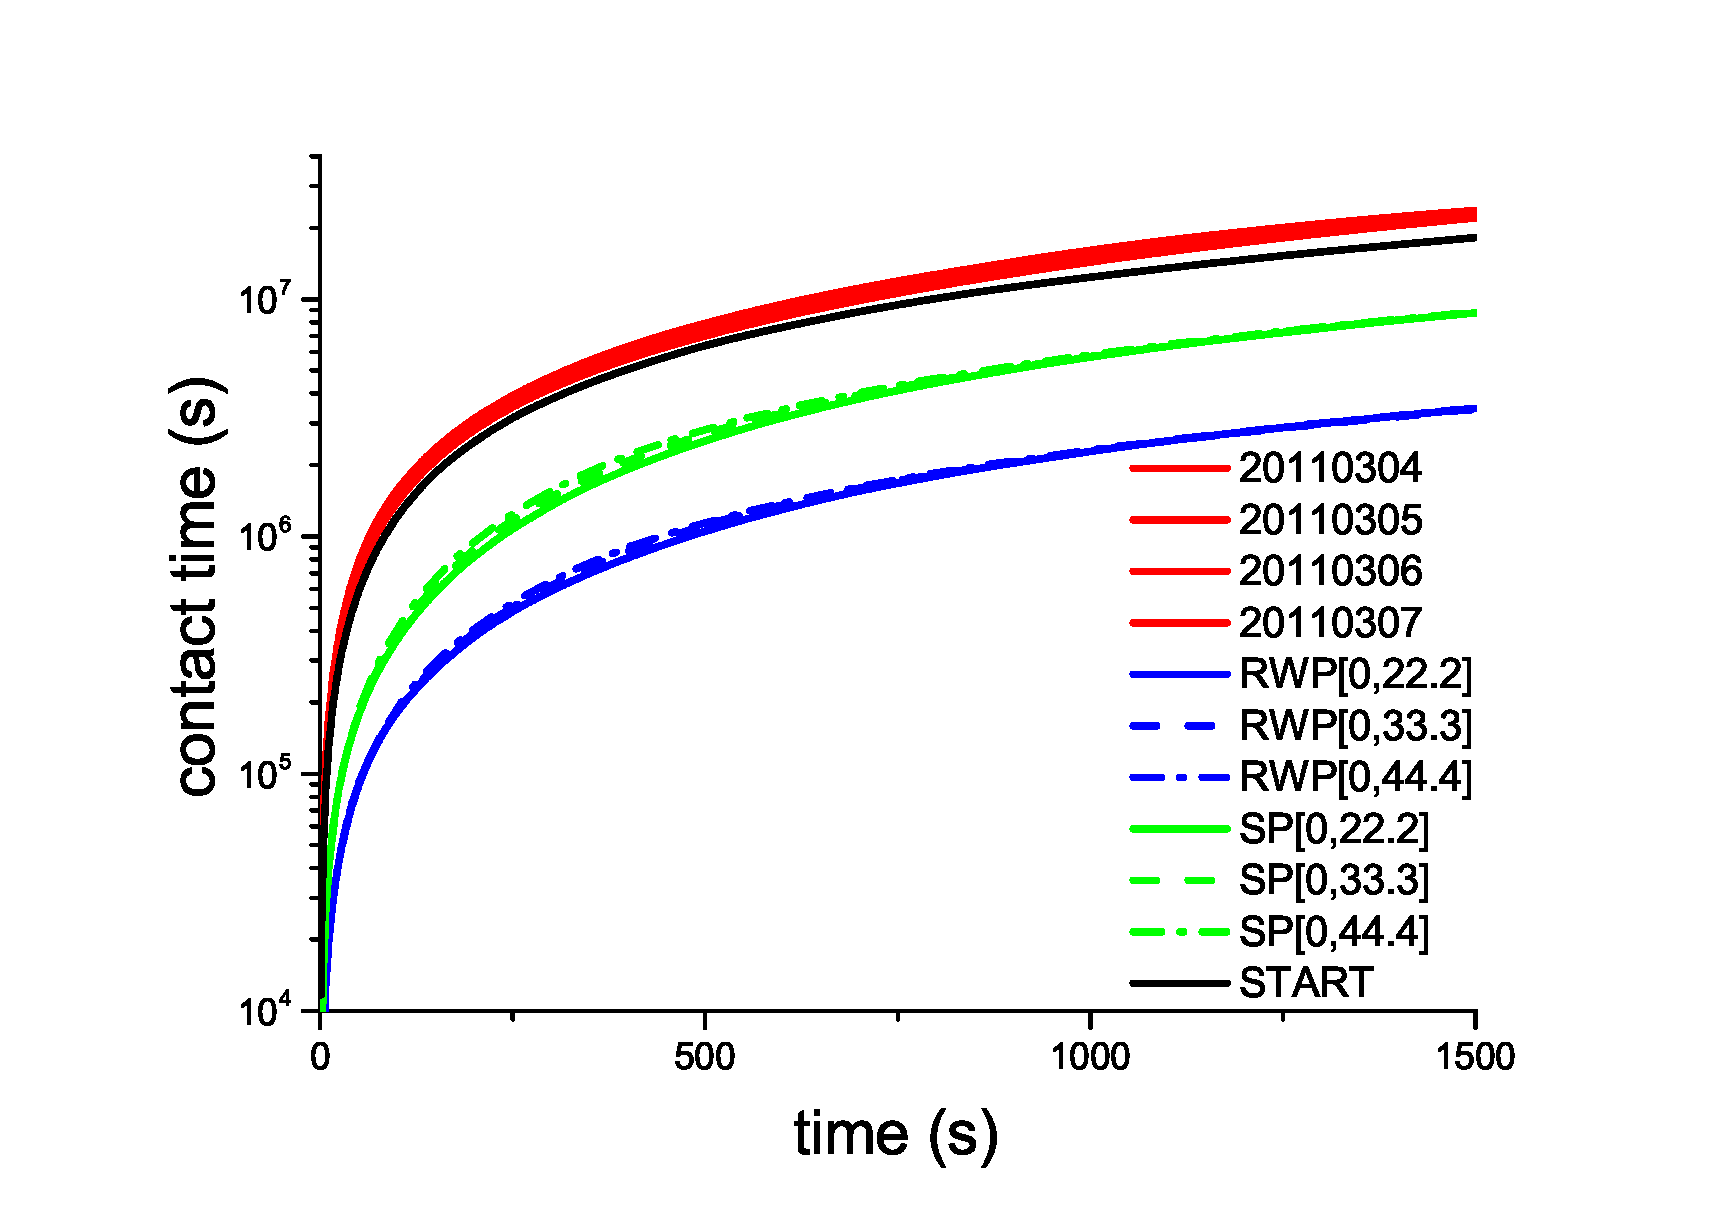
\includegraphics[width=0.23\textwidth]{figures_201103/Evaluation/contact/tc_logscale.eps}}
\caption{time vs. total contact time}\label{figure_total_contact_time}
\end{figure}

Fig. \ref{figure_contacts}. (a)(b) is the contact time and inter-contact distribution, which shows the probability of the contact or inter-contact time smaller than certain time length. To substantiate, a point $(200,0.5)$ in these figures means the probability is 0.5 when contact or inter-contact time is shorter than $200s$. In addition, a point $(x,y)$ in \ref{figure_total_contact_time}.(a) means the sum of contact time is y when the simulation time is x. In this figure, the three green lines of SP and the three blue lines of RWP are coincide with each other. To recognize the differences, we set y axis as log-scale in fig.\ref{figure_total_contact_time}.(b).
The curves of the total contact time vs. time presents a liner law. For SP and RWP, the differences of speed ranges show little influence on these curves.
Clearly, the rank of the contact characteristic similarity with the real data is $START>SP>RWP$.

To conclude, by comparing the node distribution and contact characteristics, the START mobility model performs good similarity with the real data.The evaluation results conform to our expectations. Because $START$ takes use of speed and geographic feathers related with status, While SP employs the map information and RWP is a random model taking use of no realistic data.

